%%%%%%%%%%%%%%%%%%%%%%%%%%%%%%%%%%%%%%%%%%%%%%%%%%%%%%%%%%%%%%%%%%%%%%%%%%%%%%%%%%
\begin{frame}[fragile]\frametitle{}

\begin{center}
{\Large Notes from ``The Master Algorithm'' - Pedro Domingos}

  {\tiny (Ref: Pedro Domingos: "The Master Algorithm" | Talks at Google)}

\end{center}


\end{frame}

%%%%%%%%%%%%%%%%%%%%%%%%%%%%%%%%%%%%%%%%%%%%%%%%%%%%%%%%%%%%%%%%%%%%%%%%%%%%%%%%%%
\begin{frame}[fragile]\frametitle{The book is \ldots}
  \begin{itemize}
    \item All about``Machine Learning''
	\item Today there are five tribes (as categorized by Domingos), each with their own master algorithm. 
	\item Best for itself but not for others.
	\item The ultimate master algorithm combines them into a general purpose learning machine.
  \end{itemize}
\end{frame}

%%%%%%%%%%%%%%%%%%%%%%%%%%%%%%%%%%%%%%%%%%%%%%%%%%%%%%%%%%%%%%%%%%%%%%%%%%%%%%%%%%
\begin{frame}[fragile]\frametitle{The Origins of Human Knowledge}
  \begin{itemize}
    \item Evolution:  Knowledge encoded in our DNA that makes us what we are. Built through Survival of Fittest.
	\item Experience: Acquired by living in the world.
	\item Culture: from culture, from talking with other people, from reading books and so on.
	\end{itemize}

	These are the sources of knowledge in natural intelligence. The next one far better than the previous one.
	
	There is a new source of knowledge on the planet and that’s \ldots
	
	
  {\tiny (Ref: Shane Parrish Blog)}
  
\end{frame}

%%%%%%%%%%%%%%%%%%%%%%%%%%%%%%%%%%%%%%%%%%%%%%%%%%%%%%%%%%%%%%%%%%%%%%%%%%%%%%%%%%
\begin{frame}[fragile]\frametitle{The Origins of Human Knowledge}
Computers \ldots

  \begin{itemize}
    \item Discovering knowledge from data.
	\item for example, these days there are hedge funds that are completely run by machine learning algorithms. 
	\item They look at the data, they make predictions and they make buy and sell decisions based on those predictions. 
	\end{itemize}

 \begin{center}
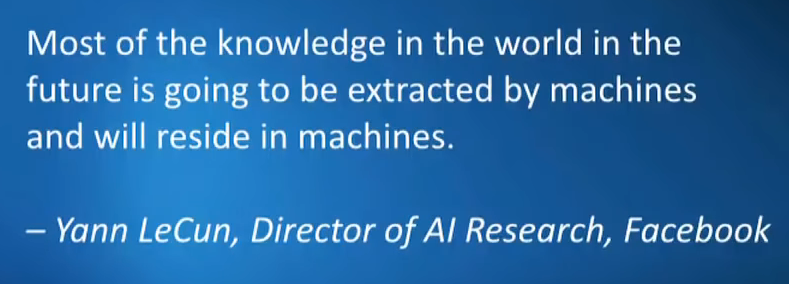
\includegraphics[width=0.5\linewidth,keepaspectratio]{masteralgo3}
\end{center}

  
\end{frame}

%%%%%%%%%%%%%%%%%%%%%%%%%%%%%%%%%%%%%%%%%%%%%%%%%%%%%%%%%%%%%%%%%%%%%%%%%%%%%%%%%%
\begin{frame}[fragile]\frametitle{5 main paradigms in Machine Learning}
COmputers discover knowledge by mimicking following processes:
  \begin{itemize}
    \item Filling Gaps: Scientists put forth hypothesis/theories, make observations, adapt the theory to fill the gap.
	\item Reverse Engineering: Emulate the brain. The greatest learning machine on earth is under your skull.
	\item Simulate Evolution: More superior than brain, as it creates brain, body, other life forms, etc.
	\item Quantify uncertainty/probability: As more evidence comes, adjust it, using Bayes' theorem.
	\item Reason by analogy: You try to find matching similar situation from past, apply its solution.
  \end{itemize}
  
  For each of these, there is a school of thought \ldots
\end{frame}

%%%%%%%%%%%%%%%%%%%%%%%%%%%%%%%%%%%%%%%%%%%%%%%%%%%%%%%%%%%%%%%%%%%%%%%%%%%%%%%%%%
\begin{frame}[fragile]\frametitle{5 Tribes}
  \begin{itemize}
    \item Symbolists: Learning as the inverse of deduction
	\item Connectionists: Reverse engineer the brain, seen in back-propagation
	\item Evolutionaries: Simulate evolution on the computer, seen in genetic programming
	\item Bayesians: A form of probabilistic inference
	\item Analogizers: Extrapolating from similarity judgments, seen in Support vector machines.
  \end{itemize}
  
  Each of these have their own master algorithm, to learn ANLYTHING (given enough data, proof available).
\end{frame}

%%%%%%%%%%%%%%%%%%%%%%%%%%%%%%%%%%%%%%%%%%%%%%%%%%%%%%%%%%%%%%%%%%%%%%%%%%%%%%%%%%
\begin{frame}[fragile]\frametitle{Symbolists}
  \begin{itemize}
    \item Filling in the gaps of the knowledge we have
	\item Believe in the power of logic
	\item Master Algorithm: Inverse deduction
	\item Famous folks:
	
	 \begin{center}
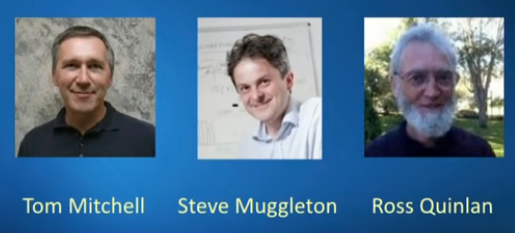
\includegraphics[width=0.5\linewidth,keepaspectratio]{masteralgo4}
\end{center}

  \end{itemize}


  
\end{frame}

%%%%%%%%%%%%%%%%%%%%%%%%%%%%%%%%%%%%%%%%%%%%%%%%%%%%%%%%%%%%%%%%%%%%%%%%%%%%%%%%%%
\begin{frame}[fragile]\frametitle{Inverse Deduction}
  \begin{itemize}
    \item Learning is induction of knowledge
	\item Deduction is ``general rule to specific facts''
	\item Induction is ``specific facts to general rule''
	\item Example: Addition: If I add 2 and 2, what do I get? : 4
	\item Subtraction gives answer to the inverse question: What do I add to 2 to make it 4? : 2
	\item Similarly, inverse deduction gives, what else do you need to know, to come to the answer
	\item  A general rule : ``Humans are mortal''
  \end{itemize}
  
\begin{center}
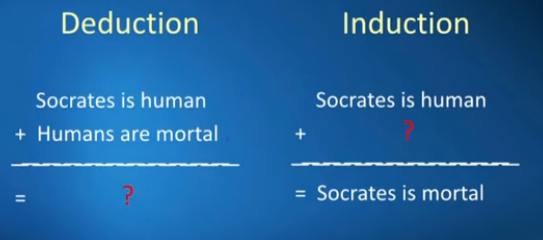
\includegraphics[width=0.5\linewidth,keepaspectratio]{masteralgo5}
\end{center}

Rules can be composed into much more complex system to match multitudes of answers.

Thats the Machine Learning!! finding the formula/function/rule given inputs and output.
  
\end{frame}

%%%%%%%%%%%%%%%%%%%%%%%%%%%%%%%%%%%%%%%%%%%%%%%%%%%%%%%%%%%%%%%%%%%%%%%%%%%%%%%%%%
\begin{frame}[fragile]\frametitle{Connectionists}
  \begin{itemize}
    \item Take their inspiration from the workings of the brain. Neural Networks.
	\item Master Algorithm: Backpropagation.
	\item Famous folks:
	
	 \begin{center}
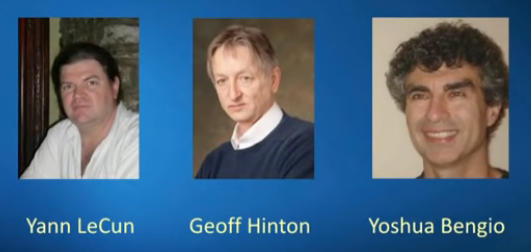
\includegraphics[width=0.5\linewidth,keepaspectratio]{masteralgo6}
\end{center}
	
  \end{itemize}


\end{frame}


%%%%%%%%%%%%%%%%%%%%%%%%%%%%%%%%%%%%%%%%%%%%%%%%%%%%%%%%%%%%%%%%%%%%%%%%%%%%%%%%%%
\begin{frame}[fragile]\frametitle{Working of Neurons}
  \begin{itemize}
	\item A neuron gets various inputs. If the weighted total crosses the threshold, it fires, and sends electrochemical signal downstream to the connected neurons.
	\item The connections are called, synapse. Stronger they are more weights, threshold crossings are  more, more transmissions happen, more learning.
	\item What we thought is not the actual, we correct our understanding, thats how we learn.
	\item Same thing happens as Back-propagation, which adjusts the weights. So that only correct neurons (branches) fire.
	
  \end{itemize}

Thats Deep learning!!
\end{frame}


%%%%%%%%%%%%%%%%%%%%%%%%%%%%%%%%%%%%%%%%%%%%%%%%%%%%%%%%%%%%%%%%%%%%%%%%%%%%%%%%%%
\begin{frame}[fragile]\frametitle{Evolutionaries}
  \begin{itemize}
    \item Learn the structure itself. Not need to feed it like Neural networks do.
	\item Test learning algorithms by their “fitness”, a scoring function as to how well the algorithm meets its purpose.
	\item The successful algorithms are then mutated and recombined (sex) to produce new algorithms that can continue the competition for survival. 
	\item Eventually an algorithm will find a fitness peak where further mutations or recombination do not increase the algorithm’s success.
	\item Master Algorithm: Genetic Programming
	
	\item Famous folks:
	
	 \begin{center}
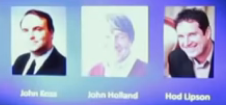
\includegraphics[width=0.5\linewidth,keepaspectratio]{masteralgo7}
\end{center}	
  \end{itemize}

Thats Genetic Programming!!

\end{frame}

%%%%%%%%%%%%%%%%%%%%%%%%%%%%%%%%%%%%%%%%%%%%%%%%%%%%%%%%%%%%%%%%%%%%%%%%%%%%%%%%%%
\begin{frame}[fragile]\frametitle{Connectionists vs Evolutionaries}
  \begin{itemize}
    \item Neural networks start with a predetermined structure. Genetic algorithms can learn their structure (although a general form would be specified). 
	\item Backpropogation, the staple process by which neural networks are trained, starts from an initial random point for a single hypothesis but then proceeds deterministically in steps to the solution. 
	\item A genetic algorithm has a sea of hypotheses competing at any one moment, with the randomness of mutation and sex potentially producing big jumps at any point, but also generating many useless algorithm children.
  \end{itemize}

{\tiny (Ref: Jason Collins Blog)}
\end{frame}

%%%%%%%%%%%%%%%%%%%%%%%%%%%%%%%%%%%%%%%%%%%%%%%%%%%%%%%%%%%%%%%%%%%%%%%%%%%%%%%%%%
\begin{frame}[fragile]\frametitle{Bayesians}
  \begin{itemize}
    \item Start with a set of hypotheses that could be used to explain the data, each of which has a probability of being true (their ‘priors’). 
	\item Those hypotheses are then tested against the data, with those hypotheses that better explain the data increasing in their probability of being true, and those that can’t decreasing in their probability. 
	\item This updating of the probability is done through Bayes’ Rule.
	\item Famous folks:
	
	 \begin{center}
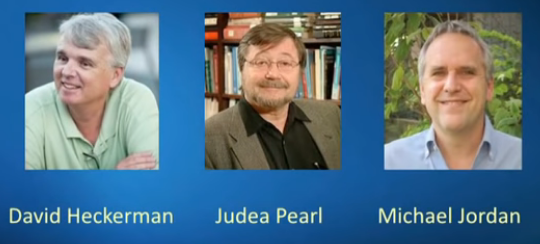
\includegraphics[width=0.5\linewidth,keepaspectratio]{masteralgo8}
\end{center}	
  \end{itemize}

\end{frame}

%%%%%%%%%%%%%%%%%%%%%%%%%%%%%%%%%%%%%%%%%%%%%%%%%%%%%%%%%%%%%%%%%%%%%%%%%%%%%%%%%%
\begin{frame}[fragile]\frametitle{What is Bayesian Learning?}
  \begin{itemize}
	    \item Everything that you learn is uncertainty/probability. Compute the probability of your hypothesis and update it as the new evidence comes in using Bayes theorem.
\item Master Algorithm:	Bayes Theorem
\item Likelihood: If your hypothesis is such that it makes observations likely, then conversely, what you are observing is what makes your hypothesis likely.

  \end{itemize}

	 \begin{center}
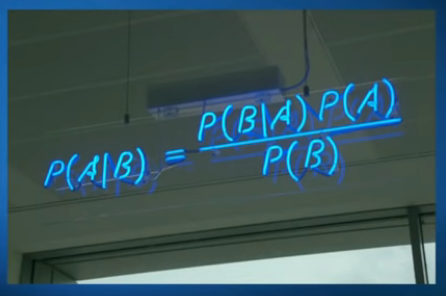
\includegraphics[width=0.35\linewidth,keepaspectratio]{masteralgo9}
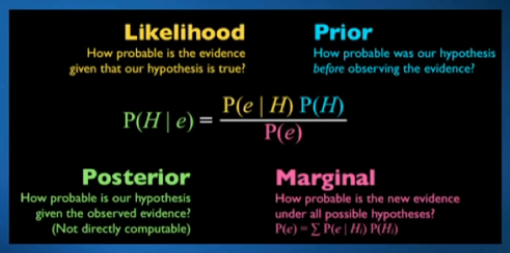
\includegraphics[width=0.55\linewidth,keepaspectratio]{masteralgo10}
\end{center}
  
\end{frame}

%%%%%%%%%%%%%%%%%%%%%%%%%%%%%%%%%%%%%%%%%%%%%%%%%%%%%%%%%%%%%%%%%%%%%%%%%%%%%%%%%%
\begin{frame}[fragile]\frametitle{Analogisers}
  \begin{itemize}
    \item Reason by analogy:apply solution of the problem in past, that matches with the current ones.
	\item Master Algorithm: KNN, Support Vector Machines.
	\item KNN can form a complicated partition. One interesting fact that, points, away from partitions are irrelevant. Only near the boundary control it. These are same as Support vectors. Same as SVM with Kernel trick.
	\item Famous folks:
	
	 \begin{center}
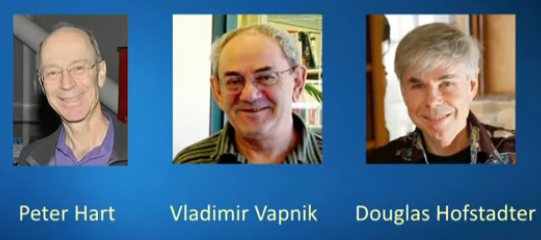
\includegraphics[width=0.5\linewidth,keepaspectratio]{masteralgo11}
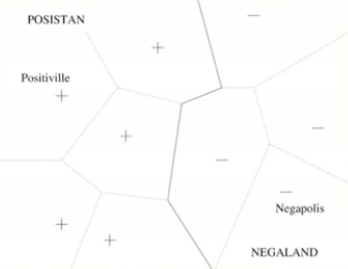
\includegraphics[width=0.4\linewidth,keepaspectratio]{masteralgo12}

\end{center}		
  \end{itemize}

\end{frame}


%%%%%%%%%%%%%%%%%%%%%%%%%%%%%%%%%%%%%%%%%%%%%%%%%%%%%%%%%%%%%%%%%%%%%%%%%%%%%%%%%%
\begin{frame}[fragile]\frametitle{Summary of Tribes}
 
 \begin{center}
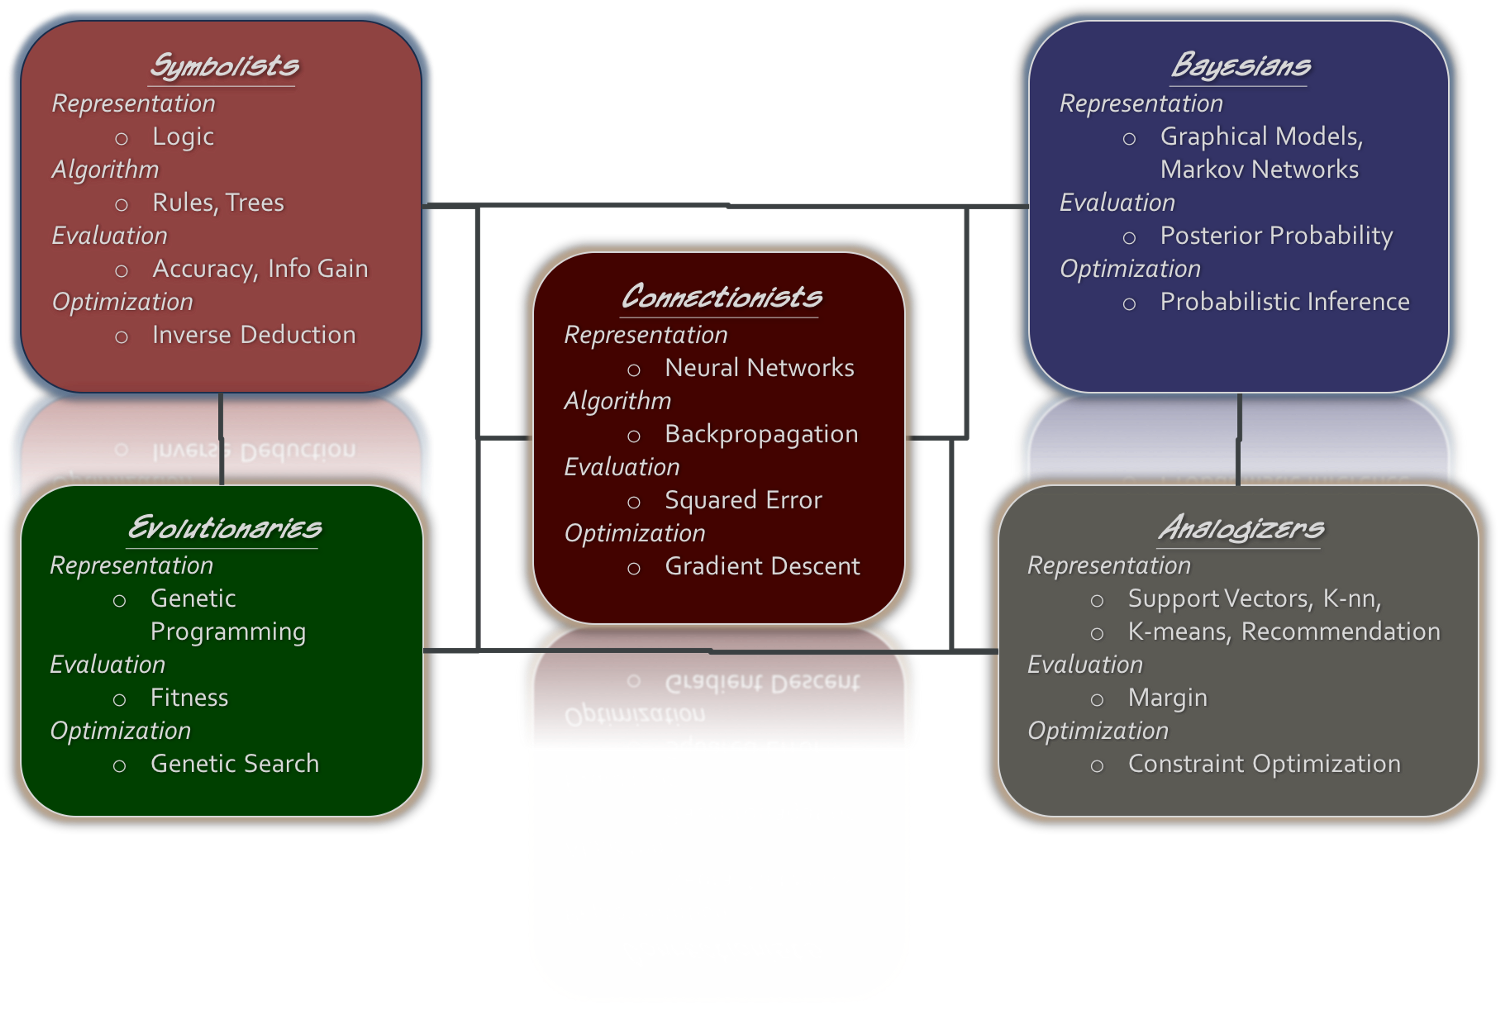
\includegraphics[width=\linewidth,keepaspectratio]{masteralgo2}
\end{center}
\end{frame}


%%%%%%%%%%%%%%%%%%%%%%%%%%%%%%%%%%%%%%%%%%%%%%%%%%%%%%%%%%%%%%%%%%%%%%%%%%%%%%%%%%
\begin{frame}[fragile]\frametitle{Summary of Tribes}
 
 \begin{center}
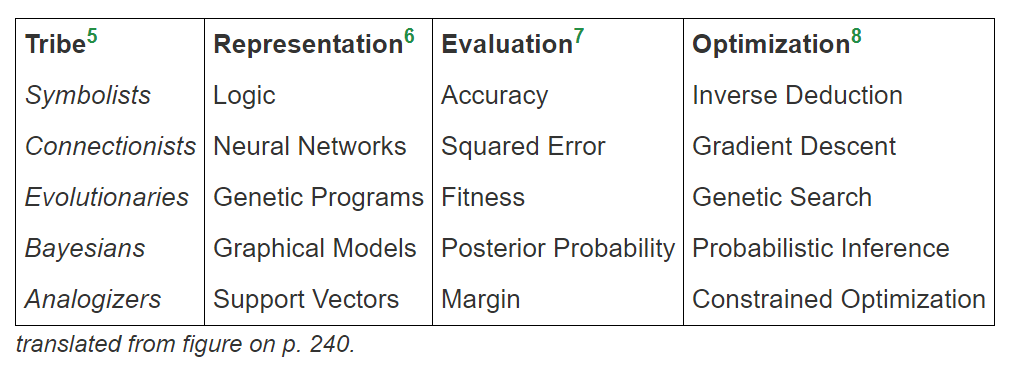
\includegraphics[width=\linewidth,keepaspectratio]{masteralgo1}
\end{center}

But we need a single algorithm that solves all of these \ldots

Thats the Master Algorithm, a Grand Unified Theory of Machine Learning.
\end{frame}



%%%%%%%%%%%%%%%%%%%%%%%%%%%%%%%%%%%%%%%%%%%%%%%%%%%%%%%%%%%%%%%%%%%%%%%%%%%%%%%%%%
\begin{frame}[fragile]\frametitle{What is The Master Algorithm?}
{\it 

``a general-purpose learner” (p. xxi) \ldots an algorithm that, ``if it exists, [it] 
can derive all knowledge in the world—past, present, and 
future—from data'' (p. xviii) \ldots 
an algorithm that can “learn to simulate any other algorithm by 
reading examples of its input-output behavior” (p. 34) \ldots
 ``the unifier of machine learning: it lets any application use any learner, 
 by abstracting the learner into a common form that is all the applications need to know'' (p. 237).
}

What a promise!!!
\end{frame}

%%%%%%%%%%%%%%%%%%%%%%%%%%%%%%%%%%%%%%%%%%%%%%%%%%%%%%%%%%%%%%%%%%%%%%%%%%%%%%%%%%
\begin{frame}[fragile]\frametitle{How can we combine all these algorithms?}
They all have same three parts:
  \begin{itemize}
    \item Unifying Representation: Markov Logic networks, rules with probability/weights.
	\item Evaluation: A scoring function that declares how good the model is. How does it fit data? How well it answers accurately? Given by the consumer, we need to optimize it.
	\item Optimization: How to optimize the model/function. Use Genetic process or crossing, come up with different combination and see which one works.
  \end{itemize}

\begin{center}
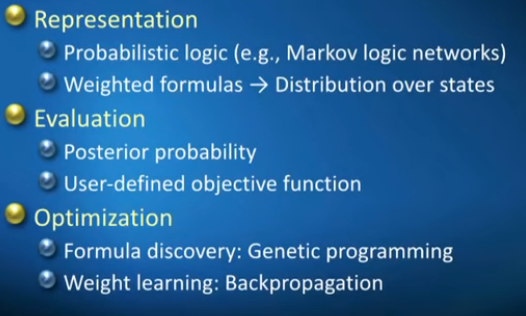
\includegraphics[width=0.5\linewidth,keepaspectratio]{masteralgo13}
\end{center}

\end{frame}


